% !TEX root = ../thesis-example.tex
%
\chapter{Obrazowanie OCT}
\label{sec:obrazowanie_oct}

% Wstęp do OCT

\textbf{Optyczna tomografia koherencyjna} (ang. \textit{optical coherence tomography, OCT}) jest metodą umożliwiającą nieinwazyjne oraz \textit{in vivo} przechwycenie obrazu wnętrza tkanki biologicznej. Zasada działania OCT opiera się na wykorzystaniu fal świetlnych. Dzięki temu rozdzielczość obrazów jest o wiele wyższa niż w ultrasonografii (wykorzystanie fal dźwiękowych), czy rezonansie magnetycznym (wykorzystanie pola magnetycznego). Następnym powodem dużej popularności OCT w medycynie jest bezkontaktowe badanie pacjenta oraz brak wymogu przygotowania pacjenta przed badaniem. 

W projekcie RIMO OCT zostało wykorzystane do uzyskania szczegółowych obrazów naczyń krwionośnych siatkówki oka. Rysunek \ref{fig:obrazowanie_oct:bscan_vessels} przedstawia przykładowe obrazy siatkówki oka uzyskane dzięki wykorzystaniu OCT. Jednym z tych przykładowych obrazów jest angiografia siatkówki oka, która jest obrazem wejściowym do algorytmów omawianych w niniejszej pracy. Sposób powstania angiografii z danych OCT jest wyjaśniony w podrozdziale \ref{sec:obrazowanie_oct:angiografia_oct}, natomiast ogólna zasada działania OCT jest wyjaśniona w podrozdziale \ref{sec:obrazowanie_oct:metoda_oct}. Na koniec rozdziału w podrozdziale \ref{sec:obrazowanie_oct:zastosowania_oct} zostaną opisane zastosowania OCT.

\begin{figure}[htb]
	\centering
	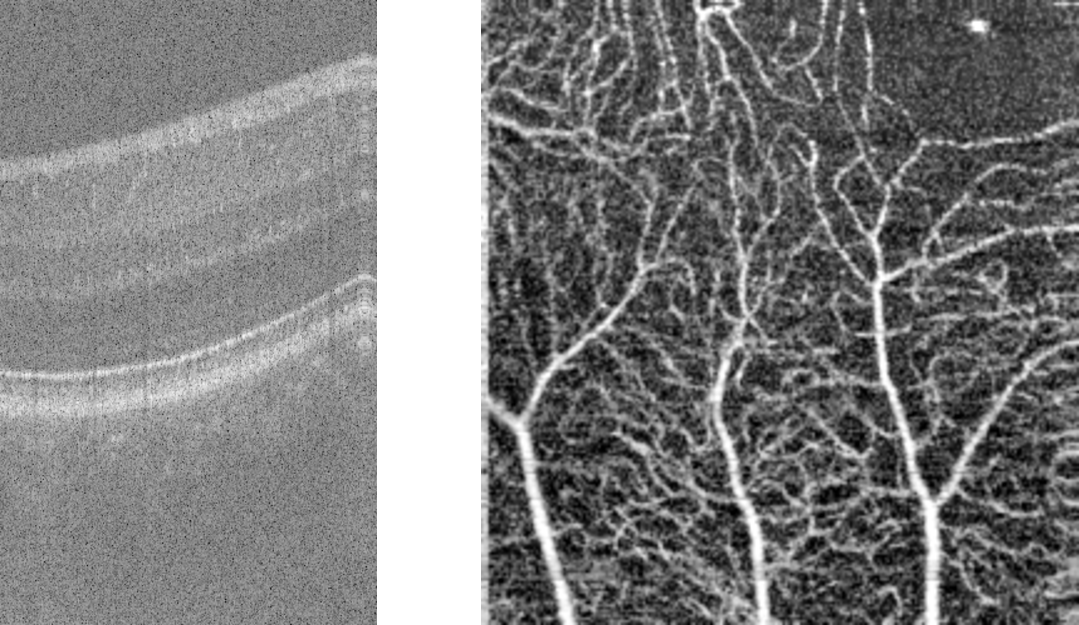
\includegraphics[width=\textwidth]{gfx/bscan_vessels}
	\caption{\textbf{Lewy obraz:} Dwuwymiarowy przekrój siatkówki oka (B-skan). Obraz został uzyskany poprzez połączenie jednowymiarowych A-skanów, które zawierają informację o strukturze tkanki w głąb siatkówki oka. \textbf{Prawy obraz:} Angiografia siatkówki oka uzyskana dzięki przetworzeniu danych z OCT.}
	\label{fig:obrazowanie_oct:bscan_vessels}
\end{figure}

% Wyjaśnia zasadę działania OCT, bez wchodzenia w duże teoretyczne detale

\section{Zasada działania OCT}
\label{sec:obrazowanie_oct:metoda_oct}

Jednym z najważniejszych parametrów metod tomografii w medycynie jest ich rozdzielczość. Optyczna tomografia koherencyjna przechwytuje obrazy wnętrza tkanki poprzez wykorzystanie fal świetlnych. OCT za pomocą generatora wytwarza falę świetlną, która jest skierowana na tkankę pacjenta. Następnie po odbiciu fali poprzez tkankę wiązka jest przechwycona przez detektor. Jedną z dostępnych metod, która umożliwiłaby zlokalizowanie miejsca odbicia fali byłoby zmierzenie czasu pomiędzy wygenerowaniem fali, a zarejestrowaniem jej przez detektor (mechanizm stosowany np. w ultrasonografii z wykorzystaniem fal dźwiękowych), natomiast prędkość światła (\(3\times10^8 \frac{m}{s}\)) wyklucza zastosowanie tego mechanizmu. Zjawisko, które umożliwia dokładne zlokalizowanie miejsca odbicia to \textbf{interferencja światła o niskiej spójności}.

\begin{figure}[htb]
	\centering
	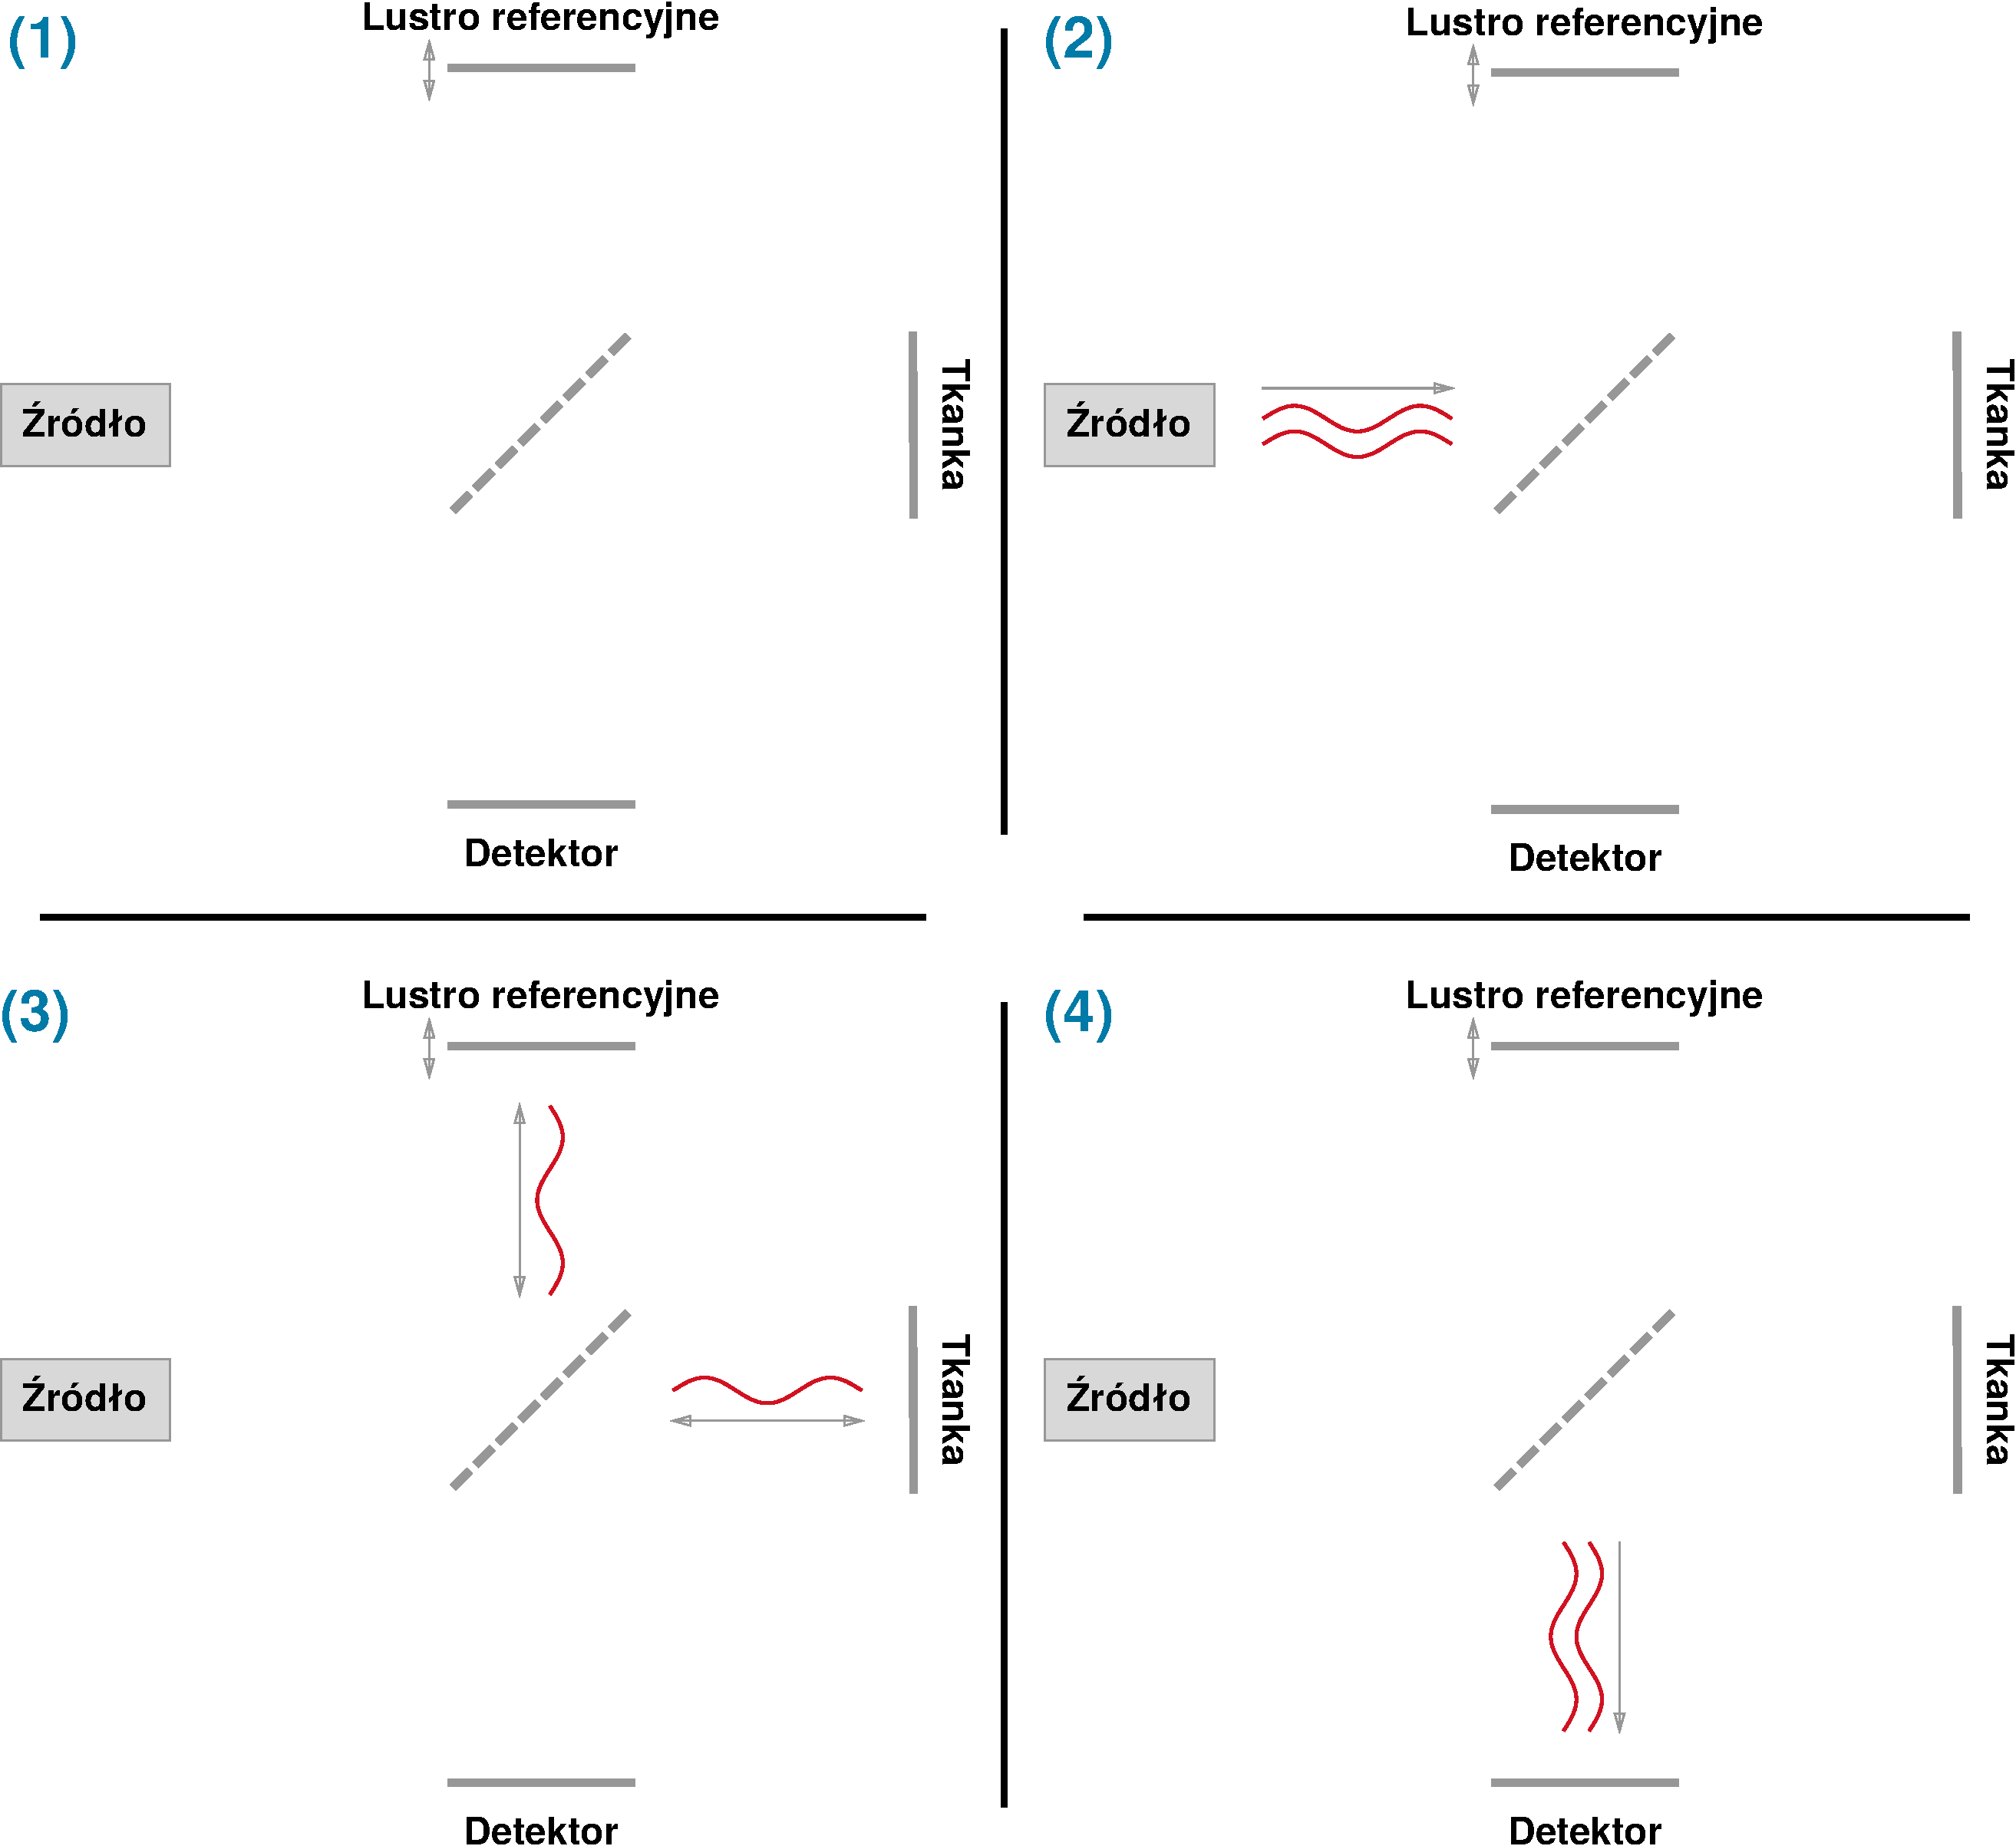
\includegraphics[width=\textwidth]{gfx/oct_phases}
	\caption{Kolejne etapy działania metody OCT. \textbf{(1)} - Etap początkowy. \textbf{(2)} - Źródło wyemitowało wiązkę światła. \textbf{(3)} - Fala rozdzieliła się za pomocą interferometru na wiązkę referencyjną (skierowaną na lustro referencyjne) oraz na wiązkę próbki (skierowaną na tkankę). \textbf{(4)} - Wiązki po odbiciu od lustra referencyjnego i tkanki ponownie łączą się za pomocą interferometru. W tej części występuje zjawisko interferencji, które jest zarejestrowane przez detektor.}
	\label{fig:obrazowanie_oct:oct_phases}
\end{figure}

Rysunek \ref{fig:obrazowanie_oct:oct_phases} składa się z bardzo uproszczonych schematów OCT, które obrazują kolejne etapy działania metody. Schematy na rysunku \ref{fig:obrazowanie_oct:oct_phases} składają się z pięciu elementów:

\begin{itemize}

\item \textbf{Źródła} - Źródło (np. dioda superluminescencyjna) światła podczerwonego, które jest falą o niskiej spójności.
\item \textbf{Rozdzielacza wiązek} (na rysunku \ref{fig:obrazowanie_oct:oct_phases} przedstawiony za pomocą przerywanych linii na środku każdego schematu) - Interferometr (np. Michelsona) umożliwiający rozdzielenie fali na dwie wiązki oraz następne ich połączenie.
\item \textbf{Lustro referencyjne} - Lustro, które odbija wiązkę referencyjną. Posiada możliwość oddalania oraz przybliżania się względem interferometru.
\item \textbf{Tkanka} - Badana tkanka, która odbija wiązkę próbki.
\item \textbf{Detektor} - Rejestruje zjawisko interferencji związek.

\end{itemize}

Najbardziej istotnym etapem wymaganym do zrozumienia mechanizmu OCT jest etap (4) pokazany na rysunku \ref{fig:obrazowanie_oct:oct_phases}. W tym kroku wiązka referencyjna i wiązka próbki łączą się i zachodzi zjawisko interferencji. Dzięki temu, że wiązki są falami o niskiej spójności interferencja zachodzi tylko na małej długości (ang. \textit{coherence length}). Odczytując za pomocą detektora charakterystyczny wzorzec interferencji występującej na \textit{coherence length} jesteśmy w stanie wydobyć informacje na temat próbki wnętrza tkanki oraz wiemy dzięki położeniu lustra referencyjnego położenie próbki. Poszczególne badanie głębszych warstw tkanki przedstawia rysunek \ref{fig:obrazowanie_oct:tissue_layers}.

\begin{figure}[htb]
	\centering
	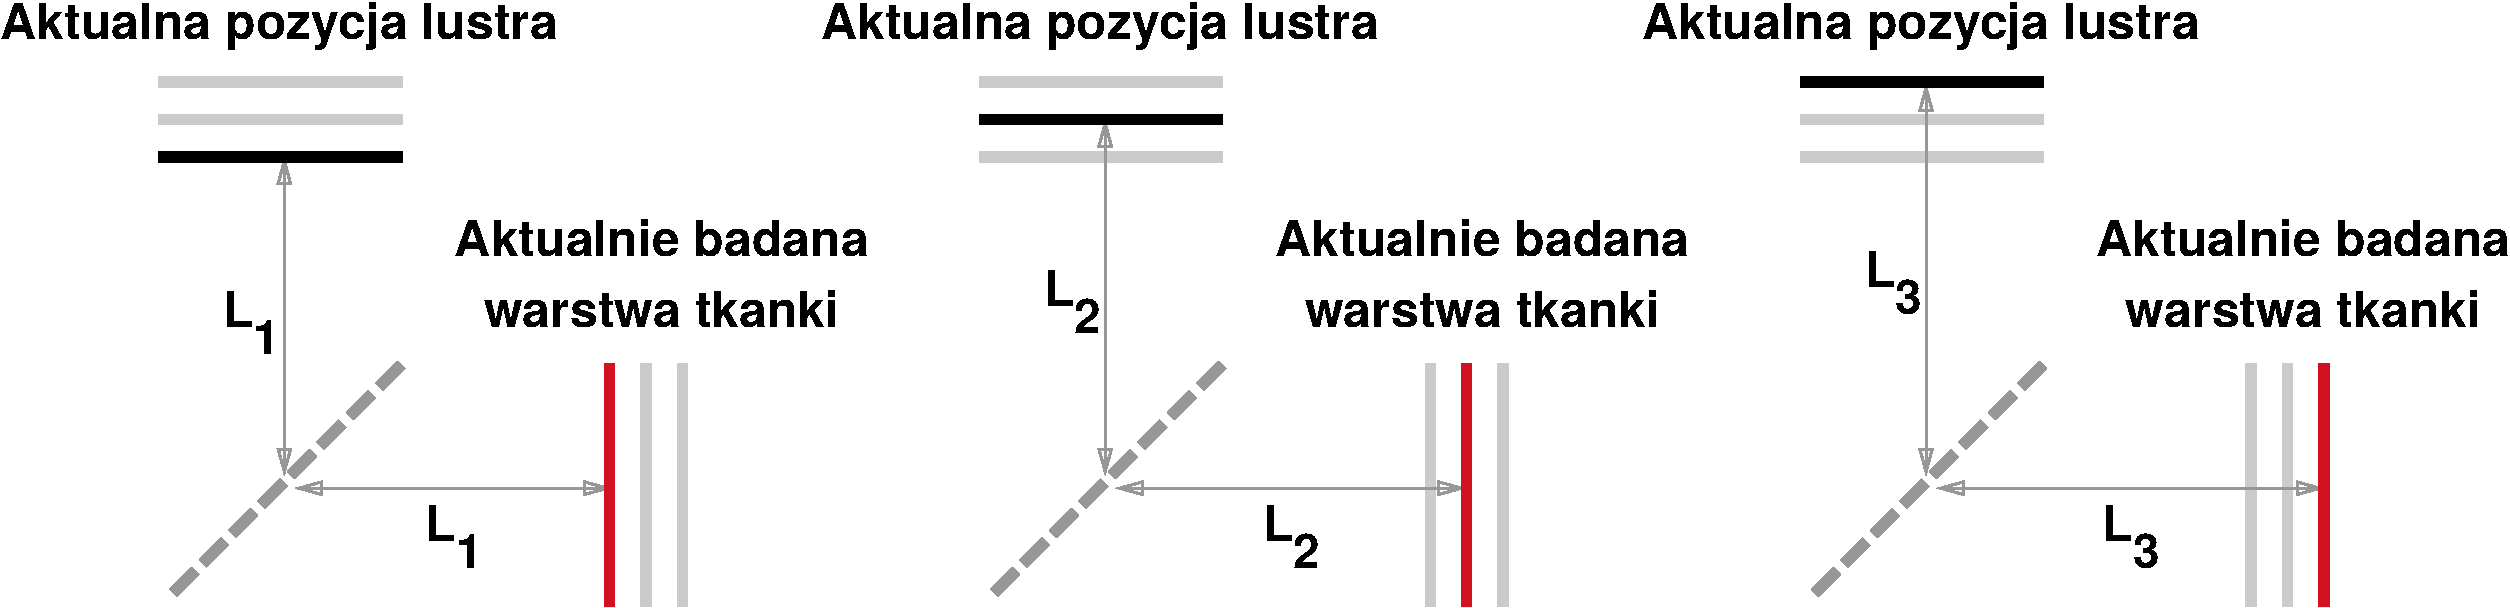
\includegraphics[width=\textwidth]{gfx/tissue_layers}
	\caption{Kolejne etapy badania głębszych warstw tkanki dzięki przesuwaniu lustra referencyjnego. Aktualna pozycja lustra referencyjnego jest zaznaczona kolorem czarnym, natomiast aktualnie badana warstwa tkanki jest zaznaczona kolorem czerwonym.}
	\label{fig:obrazowanie_oct:tissue_layers}
\end{figure}

\subsection{Uzyskanie całościowego obrazu tkanki}

Poprzez poruszenie lustra referencyjnego pomiary przeprowadzane są w głąb tkanki (wzdłuż osi Z). Zbiór pomiarów w głąb tkanki nazywa się A-skanem (obraz jednowymiarowy). Powtarzając ten proces w osi X lub Y i następnie poprzez połączenie sąsiadujących A-skanów otrzymuje się przekrój tkanki zwany B-skanem (obraz dwuwymiarowy). Cały proces uzyskania B-skanów można powtórzyć dla sąsiadujących przekrojów. Poprzez połączenie otrzymanych B-skanów otrzymuje się obraz trójwymiarowy tkanki. Na rysunku \ref{fig:obrazowanie_oct:scan} \cite{Kraus:12} przedstawione są poszczególne skany.

\begin{figure}[htb]
	\centering
	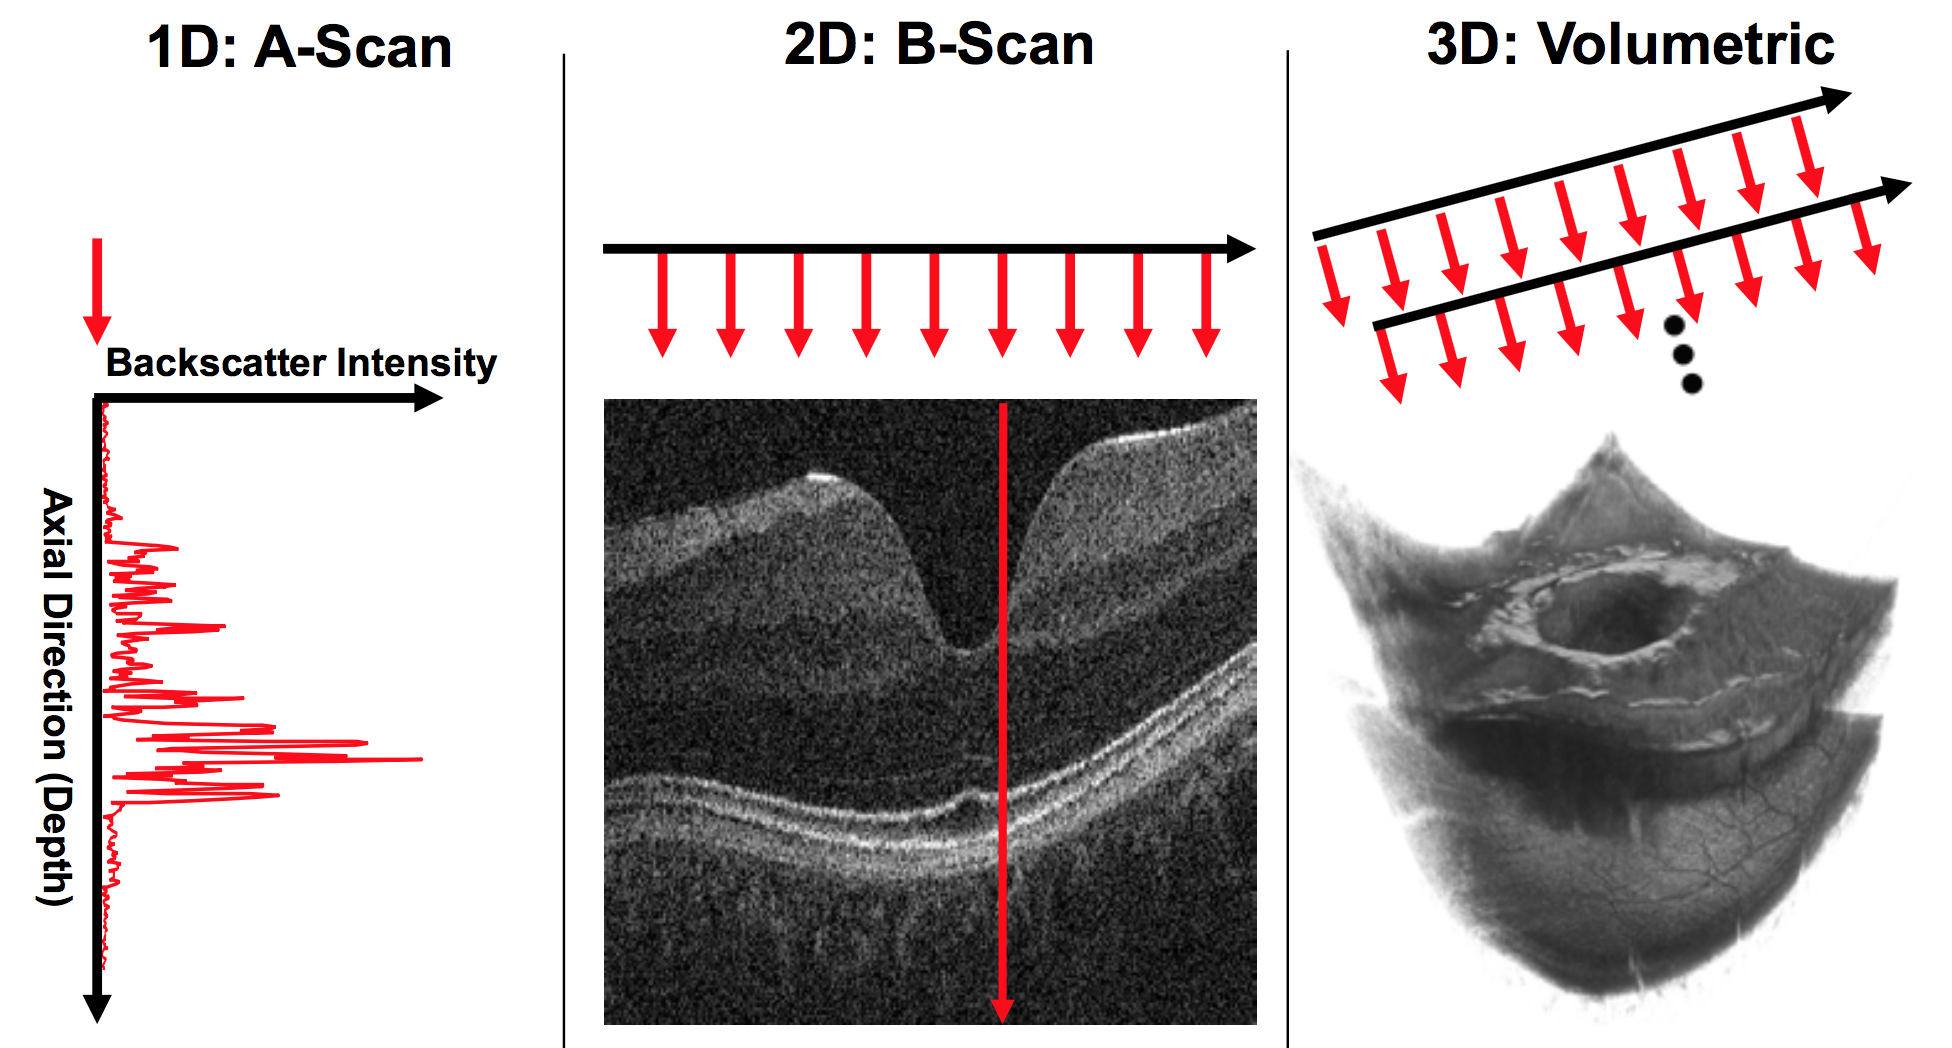
\includegraphics[width=\textwidth]{gfx/scans}
	\caption{\cite{Kraus:12} \textbf{Lewy obraz:} Pojedynczy A-skan wykonany w głąb tkanki. \textbf{Środkowy obraz:} Otrzymany B-skan poprzez połączenie A-skanów. \textbf{Prawy obraz:} Trójwymiarowy obraz tkanki stworzony poprzez połączenie B-skanów.}
	\label{fig:obrazowanie_oct:scan}
\end{figure}

\subsection{OCT w domenie częstotliwości}

Metoda OCT, która wykonuje ruch lustrem referencyjnym jest zwana metodą OCT w domenie czasu (ang. \textit{time-domain OCT, TdOCT}). Alternatywną oraz nowszą metodą od TdOCT jest OCT w domenie częstotliwości (ang. \textit{Fourier-domain OCT, FdOCT}). FdOCT umożliwia 100 razy szybsze \cite{Strong:11} skanowanie w porównaniu do TdOCT. TdOCT jest w stanie wykonać ok. 400 A-skanów w przeciągu sekundy, natomiast FdOCT jest ich w stanie wykonać dziesiątki tysięcy. Szybsze skanowanie poprawia również jakość skanów ze względu na to, że pacjent ma mniejszą szansę poruszenia okiem podczas skanowania (ruch oka w trakcie skanowania przyczynia się do powstania artefaktów ruchu na obrazach OCT). Oprócz poprawy szybkości skanowania FdOCT ma wyższą rozdzielczość w przedziale od 3-7 mikrometrów \cite{Strong:11}. Jest to poprawa względem TdOCT o 8-10 mikrometrów.

Większa szybkość oraz rozdzielczość FdOCT w porównaniu do TdOCT jest możliwa dzięki dwóm modyfikacjom technicznym:

\begin{enumerate}

\item FdOCT jako źródło światła wykorzystuje laser o wysokiej szerokości pasma, co znacząco zwiększa rozdzielczość.
\item FdOCT jako detektor wykorzystuje spektrometr, który przeprowadza analizę widma fali (połączona wiązka referencyjna i próbki), która dotarła do spektrometru z interferometru. Wykonanie transformaty Fouriera na widmie fali tworzy A-skan tkanki. Dzięki tej technice FdOCT wyeliminowało potrzebę ruszania lustrem referencyjnym co znacząco zwiększa szybkość skanowania.

\end{enumerate}

FdOCT posiada również wady. Jest droższy od TdOCT ze względu na wykorzystanie drogiego lasera jako źródła światła co powoduje, że jest wykorzystywany tylko w celach badawczych. Następna wada wynika z szybkości powstawania A-skanów. Szybsze skanowanie może prowadzić do utraty jakości obrazów OCT, natomiast utrata tej jakość może być zmniejszona poprzez użycie techniki przetwarzania sygnałów zwanej \textit{oversampling}.

% Wyjaśnia zasadę powstawania obrazów angiograficznych z danych 7OCT

\section{Angiografia OCT}
\label{sec:obrazowanie_oct:angiografia_oct}

% Opisuje zastosowania OCT

\section{Zastosowania OCT}
\label{sec:obrazowanie_oct:zastosowania_oct}

Optyczna tomografia koherencyjna ze względu na swoje właściwości (badanie nieinwazyjne oraz \textit{in vivo}) jest metodą, która ma szerokie zastosowanie w medycynie oraz w innych specjalizacjach.

\subsection{OCT w optyce}

Najbardziej popularnym zastosowaniem OCT w medycynie jest badanie oka \cite{Fercher03}. Technika OCT umożliwia przechwycenie trójwymiarowych obrazów części oka takich jak dno, czy warstwy przednie. Dzięki temu jest wykorzystywane do diagnozowania takich chorób jak stwardnienie rozsiane, zwyrodnienie plamki żółtej, czy jaskra. 

\subsection{OCT w gastroenterologi i dermatologi}

OCT w porównaniu do innych metod diagnostycznych w medycynie jest techniką nową. Lekarze i naukowcy nieustannie starają się znaleźć nowe zastosowania dla OCT, która jest metodą obiecującą i szybko rozwijającą się. OCT jest potencjalnym kandydatem by w niektórych diagnozach zastąpić konwencjonalną biopsję, która wymaga usunięcia kawałka tkanki z organizmu. Przykładem takiego zastosowania jest badanie struktury błon śluzowych i podśluzowych w układzie pokarmowym. W tym przypadku OCT dostarczyło czyste obrazy, które dostarczają lekarzom dużo diagnostycznej informacji \cite{Rollins:99}. Innym przykładem są próby wykorzystania OCT do wczesnej diagnozy raka skóry, który obecnie również diagnozowany jest poprzez biopsję. W tym przypadku OCT w obecnym stopniu zaawansowania nie jest w stanie dostarczyć na tyle dokładnych danych by stać się jedyną metodą diagnozy. Następnym przykładem zastosowania OCT w dermatologi jest diagnoza zapalnych chorób skóry \cite{Welzel01}.

\subsection{OCT w przemyśle}

OCT wykorzystywane jest również do zastosowań przemysłowych. Umożliwia badanie np. grubości materiałów \cite{walecki2006determining}, czy badanie grubości warstwy pancerza tabletek podczas ich produkcji w przemyśle farmaceutycznym \cite{markl2014device}.
















